\documentclass{article}
\usepackage[a4paper, left=2cm, right=2cm, top=1.5cm, bottom=1.5cm]{geometry}
\usepackage[heading=true, zihao=-4, UTF8]{ctex}
\usepackage{setspace}
\usepackage{graphicx}     %插入图片的宏包
\usepackage{float}        %设置图片浮动位置的宏包
\usepackage{abstract}     %设置摘要样式
\usepackage{caption}
\usepackage{fontspec}   %设置英文字体
\usepackage{titletoc}     %设置目录样式
\usepackage{amsmath}

\setmainfont{Times New Roman} %设置英文字体

\let\kaishu\relax
\newCJKfontfamily\kaishu{KaiTi}[AutoFakeBold]
\let\songti\relax
\newCJKfontfamily\songti{SimSun}[AutoFakeBold]

\ctexset{
  section = {
    format += \zihao{3} \heiti \mdseries,
    aftername = \hspace{0.5em}
  },
  subsection = {
    format += \zihao{-3} \heiti \mdseries,
    aftername = \hspace{0.5em}
  } ,
  subsubsection = {
    format += \zihao{4} \heiti \mdseries,
    aftername = \hspace{0.5em}
  }
}

\renewcommand{\contentsname}{\zihao{3}\heiti\mdseries 目\ \ \ 录}
\titlecontents{section}[0pt]{\vspace{0.25\baselineskip} \mdseries \zihao{-4}}{\contentslabel{1em}}{}{\titlerule*[0.25pc]{.} \contentspage}
\titlecontents{subsection}[2.6em]{\vspace{0.25\baselineskip} \mdseries \zihao{-4}}{\contentslabel{1.6em}}{}{\titlerule*[0.25pc]{.} \contentspage}
\titlecontents{subsubsection}[4.3em]{\vspace{0.25\baselineskip} \mdseries \zihao{-4}}{\contentslabel{2.3em}}{}{\titlerule*[0.25pc]{.} \contentspage}

\renewcommand {\thetable} {\thesection{}-\arabic{table}}    %设置表格编号与章节对应
\renewcommand {\thefigure} {\thesection{}-\arabic{figure}}  %设置图片编号与章节对应
\renewcommand {\theequation} {\thesection{}-\arabic{figure}}  %设置图片编号与章节对应

\captionsetup {
  font={
    small,
    stretch=1.25
  },
  labelsep=space
}

\begin{document}
\zihao{-4}

\pagestyle{empty} %自定义封面
\begin{center}
  {\zihao{-4} \hspace{1em} \\ \vspace{1em}}
  {\zihao{0} \songti 珠海科技学院 \\ \vspace{1em}}
  {\zihao{0} \songti \textbf{毕\ 业\ 设 \ 计} \\ \vspace{1em}}
  {\zihao{-1} \kaishu \textbf{基于FPGA的JPEG图像编解码系统设计} \\ \vspace{4em}}
  \zihao{-2}
  \kaishu
  \makebox[10em][s]{学院:}\ {\makebox[10em][l]{电子信息工程学院}}\\
  \makebox[10em][s]{专业名称:}\ {\makebox[10em][l]{微电子科学与工程}}\\
  \makebox[10em][s]{学生姓名:}\ {\makebox[10em][l]{黄智为}}\\
  \makebox[10em][s]{学号:}\ {\makebox[10em][l]{03210828}}\\
  \makebox[10em][s]{指导老师姓名、职称:}\ {\makebox[10em][l]{孙永坚\ 讲师}}\\
  \vspace{1em}
  {\zihao{4} \heiti 完成日期:\today}
\end{center}
\clearpage


\newpage
\pagestyle{plain} 
\setcounter{page}{1}
\pagenumbering{Roman}

\renewcommand{\abstractnamefont}
  {\centering\zihao{-4}\normalfont\sffamily}
  \renewcommand{\abstractname}{\zihao{3} \heiti 摘\ \ \ 要}
\begin{abstract}
  \zihao{-4}
  随着近几十年来多媒体技术、图像扫描技术、移动终端、通信技术的不断发展,数
  字图像和视频数据的广泛使用,图像数据的数量呈指数机增加。于此对图像数据的
  存储以及传输的需求日益严峻。一味地添加设备的存储容量和信道的带宽是不现实
  的,对此使用图像压缩技术来减少图像数据的数据量。而作为静态图像压缩国际标
  准格式的JPEG(Joint Photographic Experts Group),因具有压缩率高、失真率
  小等特点。在国际上取得广泛的应用。

  目前大多数的JPGE格式图像数据编解码系统都是基于软件编程从而运行在通用计算
  机上。这种方式存在计算效率低、实时性低、运行功耗高等诸多缺点。于此同时具
  有对硬件可编程、运行功耗低的FPGA(Field Programmable Gate Array)芯片的
  规模不断增加,在FPGA芯片内实现复杂的数字信号处理系统已成为现实。因此本设
  计将JPEG压缩技术和FPGA相结合提升系统的性能,并从实际工程出发,设计出一套
  JPEG编解码系统。完成JPEG编解码在FPGA上的实现。

  本论文的结构首先阐述了JPEG格式的编解码FPGA实现的研究背景与意义国内外研究
  现状,并以此提出了一种新型的基于脉动阵列实现DCT算法的流水线结构。接着描
  述了JPEG格式编码和解码算法的实现步骤。然后采用SOC的设计思想,给出整个硬
  件系统的内部结构、层次划分,对每个运算步骤进行了详细的描述。最后完成整体
  的验证。 

  本设计基于Xilinx的Zynq系列的FPGA的硬件平台,对CMOS图像传感器OV5640采集的
  图像数据进行采集和压缩,再通过使用低速串行通信协议传输压缩数据。在EDA 工
  具vivado2019.1中完成综合仿真、布局布线以及码流生成。 \vspace{1em} \\
  \noindent\textbf{\songti 关键词:} FPGA;图像压缩;JPEG
\end{abstract}

\newpage

\renewcommand{\abstractnamefont}
  {\centering\large\normalfont\sffamily}
  \renewcommand{\abstractname}{ABSTRACT}
\begin{abstract}
    this is adstract

    \noindent\textbf{keywords:} FPGA,JPEG
\end{abstract}

\newpage
\tableofcontents

\newpage
\setcounter{page}{1}
\pagenumbering{arabic}

\begin{spacing}{1.25} %设置行距离
\section{绪\ \ 论}
  \subsection{研究背景及研究意义}
  \subsubsection{选题背景}
    图像数据作为信息的重要载体,在如今这个信息化的社会扮演着不可欠缺的角色
    相对与文本,图像具有强大的表达能力,通过像素、色彩及形状结构等元素传递
    出大量的信息。随着高清图像和视频的普及,图像数据的数量呈指数级增长。对
    高存储空间传输带宽的需求日益严峻。一味地添加设备的存储容量和信道的带宽
    是不现实的,因此图像压缩技术孕育而生。

    目前图像压缩格式应用最广的是JPGE压缩格式。它运用图像数据在空间上的冗余
    性以及人眼对图像的辨别度有限等特性来减少图像的数据量。目前JPEG图像大多
    数使用软件进行编解码。但对于医疗器械、自动驾驶、视频监控等对视频画面逐
    帧处理要求高的场景,这种方式有着效率低、运行功耗高等诸多缺点。
  \subsubsection{研究意义}
    本设计采用FPGA高并行计算能力和低功耗的特性设计出一套高效运行的JPGE格式
    编解码系统。该系统能保证图像数据高实时传输地同时保持较低的功耗,适合运
    它运用在嵌入式系统或边缘计算设备。通过对算法进行硬件级优化,FPGA能够对
    JPGE压缩的各个环节进行流水线和并行处理。相对于传统的软件开发方式极大地
    提升了系统的吞吐量和响应速度,同时保持较低的运行功耗。此外这种编解码系
    统作为软核结合FPGA使用使用具有较强的可扩展性,可与大多数视频图像处理系
    统相结合,助力更多地创新应用开发。
  \subsection{国内外研究现状}
    随着近几十年来信息技术地不断发展,图像和视频数据被广泛运用。因此如何降
    低数据的存储大小和传输系统的负担一直是研究的问题。现如今图像数据压缩编
    码主要分为两种,一种是针对静止图像在空间在空间的纬度上进行压缩编码的压
    缩方式,如JPEG、JPEG-2000、JPEG-LS。另一种是针对多个数据帧在时间纬度上
    进行压缩的方式如H.264、H.256等。其中JPEG(Joint Photographic Exprts Group,
    联合专家组)标准有ISO在1991年提出,之后有相继提出了JPEG-L、JPEG-MOTION
    、JPEG2000三个图像标准,JPEG-LS是一种接近无损压缩的压缩格式,其工作简单
    高效,但是输出的编码率随原图像的改变存在较大的波动。PEG-MONTION是基于JPEG
    发展起来的,可用于动态图像的压缩,但是压缩率比较低。JPEG2000是用小波变
    换代替JPEG的离散余弦变换(DCT),在低比特率下,有更良好的图像压缩性能,
    但是算法的复杂度高,因此在一下追求低负责度的实时应用中,JPEG2000无法替
    代JPEG,在大多数的场合之下,使用JPEG就能满足需要了。

    国内在JPEG的研究和应用方向上主要都是通过软件编程运行在CPU实现的。在应用
    方面,为了解决胶囊内窥镜有效空间和电池容量以及传输实时性要求高的场景,上
    海交通大学的赵恒阳、刘华使用fpga芯片对图像进行JPEG格式的编码,以2Mbps的
    数据速率进行传输,可以达到30fps的视频刷新率。在算法改进方面杜英杰针对传统
    JPEG使用固定量表,在压缩图像的视觉质量和压缩率的制衡不能灵活调节的问题。
    提出了一种基于感知量化和统计量化的自适应量化算法,可以根据在不同频率信息
    中应用不同量化步长的方法,实现更高的压缩比和更优的图像压缩效果,并使用FPGA
    进行硬件实现。

    国外在JPEN格式编解码FPGA实现的研究现状有:里斯本高级工程学院的学者利用FPGA
    独有的硬件结构可编程的特点,使用了FPGA动态局部可重构技术,根据编码的流程
    对FPGA硬件逻辑资源进行分时复用,实现硬件资源利用最大化。采用该方案相对使
    用传统的静态解决方案在资源占用上节省了60\%,但代价是是运行速度上慢了9倍。
    Shan等人通过行列分解的方式实现2D-DCT(二维离散余弦变换),并在设计中引入
    乒乓缓存器。在运行在100MHZ的时钟信号下,针对1920*1080的图像,最快解码率
    可达到30fps的视频刷新率。Teja等人针对2D-IDCT(二维离散余弦逆变换)设计了一
    种全流水的硬件结构,同时不使用乘法器,降低了2D-IDCT模块的资源利用。
  \subsection{使用芯片简介}
    本设计使用的芯片型号是Xilinx公司Zynq-7000系列的XC7Z020-CLG484。Zynq-7000
    系列是Xilinx公司推出的全可编程片上系统(All Programmable SOC),其中包含了
    PS(Processing System,处理器系统)和PL(Programmable Logic,可编程逻辑)
    两部分。

    Zynq SoC整合了ARM双核cortex-A9处理器和FPGA架构,实际上是一个片上系统
    (System on Chip, SoC),因此使得它不仅具有FPGA在能耗、性能、硬件可编程的优
    点,同时具有处理器软件可编程的优点,以提供强大的系统性能、灵活性与可扩展性。
    该芯片的可编程逻辑部分基于Xilinx 28nm工艺的7系列FPGA。
  \subsection{开发环境}
    本设计使用的开发环境是EDA工具Vivado2019.2。
    \subsubsection{Vivado简介}
      Vivado是Xilinx公司开发的集成开发环境,用于数字设计、验证和实现FPGA和SoC解决
      方案。Vivado提供了一个全面的工具集,帮助设计者从硬件设计到软件开发的整个流
      程,包括:设计与综合、FPGA的布局布线、仿真和验证、码流生成、ILA(Integrated
       Logic Anglzer)在线调试、PS端的软件开发、IP核集成。Vivado旨在提示FPGA设计的
       效率,特别是在复杂的系统级集成和高性能应用中。它广泛运用在通信、自动化、医
       疗、汽车、芯片设计等领域。

\newpage
\section{JPEG图像压缩相关理论}
  要对一张静态图像数据进行JPEG编解码从而做到压缩和解压,需要经历多个过程。如图\ref{jpeg}
  所示。
  \begin{figure}[H]
    \centering
    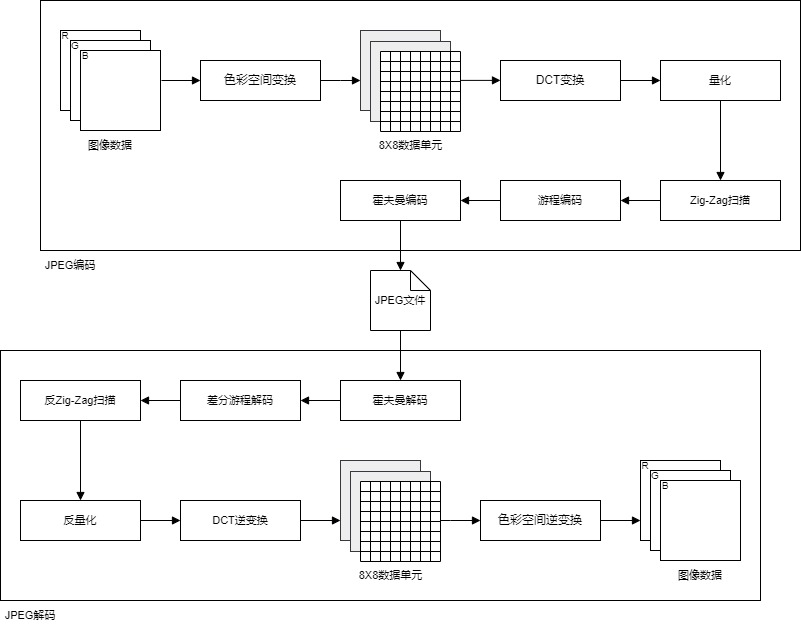
\includegraphics[scale=0.6]{./pictures/图片1.png}
    \caption{JPEG的编码和解码流程}\label{jpeg}
  \end{figure}
  JPEG格式的图像压缩流程为:首先将图像每个像素点的R、G、B颜色分量通过色彩空间变
  换转换成色度分量Cr、Cb以及亮度分量Y。之后将图片划分为若干个8*8的数据单元每个
  单元包含64个像素点,再对每个数据单元进行二维离散余弦变换(DCT),将二维的空间
  域数据变成二维的频域数据。再根据量化表对对应的频域分量进行量化处理。再通过Zig-Zag
  扫描将二维的频域数据转换成一维的序列。最后,依次通过游程编码和霍夫曼编码去除掉
  冗余的数据从而压缩JPEG图像数据。

  解压缩流程的流程与压缩的各个流程相反,除了量化和彩色空间变换这一过程会丢失一定
  的信息之外,其他的步骤都可以无损还原原数据,因此JPEG是一种有损压缩技术。

  下面依次对各个步骤做详细的描述。
  \subsection{彩色空间变换及逆变换}
    绝大多数的颜色都可以使用R、G、B三种颜色分量的线性组合进行合成。因此大多
    图像数据每个像素点都是以RGB分量表示。特别是再计算机视频技术中,不管使用
    哪种形式的彩色空间表示,最后一定要转换为RGB彩色空间显示。

    相关研究表明,人类的视觉系统有分别对红绿蓝三种颜色敏感层度的三种锥体细胞
    以及对明暗程度敏感的锥体细胞。其中对明暗程度的锥体细胞的数量大于对颜色敏
    感层度锥体细胞的数量。因此人类对是对色度辨识度大概是对明暗变换的辨识度的
    四分之一,因此可以利用对颜色感知强度的不同,将RGB彩色空间变换到YCrCb彩色
    空间再根据感知能力做对应的处理。

    ITU-R601建议规定的RGB彩色空间到YCbCr彩色空间变换关系如式\ref{RGB2YCbCr}:
    \begin{equation}
      \begin{bmatrix}Y\\ Cr\\ Cb\end{bmatrix}=
      \begin{bmatrix}
        0.299 & 0.587 & 0.144\\
        0.500 & -0.419 & -0.081\\
        -0.169 & -0.331 & 0.500
      \end{bmatrix}
      \begin{bmatrix}R\\ G\\ B\end{bmatrix}+
      \begin{bmatrix}0\\ 128\\ 128\end{bmatrix}
      \label{RGB2YCbCr}
    \end{equation}

    在JPEG编码中,RGB颜色分量的取值范围通常是0到255,因此JPEG数据使用的是8位
    无符号整数。而在YCrCb颜色空间中,色度的颜色分量Cr、Cb的范围为-128到127。为
    了将其范围转换为0到255。故添加偏移量128,以确保范围在0到255内。这有助于在
    JPEG编码和解码中正确处理色度信息。这个偏移量是JPEG编码标准的一部分,确保
    了色度信息在JPEG图像中正确显示。

    彩色空间的逆变换如下式所示:
    \begin{equation}
      \begin{bmatrix}R\\ G\\ B\end{bmatrix}=
      \begin{bmatrix}
        1 & 1.402 & 0.\\
        1 & -0.344 & -0.714\\
        1 & 0 & 0.500
      \end{bmatrix}
      \begin{bmatrix}Y\\ Cb\\ Cr\end{bmatrix}+
      \begin{bmatrix}128\\ 128\\ 128\end{bmatrix}
      \label{YCbCr2RGB}
    \end{equation}

    由于人类的视觉系统对色度变化的感知低于亮度,因此在对色度分量进行采样的时
    候可以有选择性地进行降采样,进而降低数据量,这也是最朴素的图像压缩技术之
    一。根据对色度分量的采样率不同分为一下几种采样格式:
     
    YCbCr444:每个分量的采样率都为1。这意味着对于每一个像素点都进行完整的采
    样,携带完整的原图片信息,没有信息丢失。因此YCbCr44也是最高质量的采样格
    式。

    YCbCr422:在每两个水平相邻的像素中,只用一个Cr分量和一个Cb分量来表示该这
    两个像素点的色度分量,而每一个像素点都与之对应的Y分量。这种降采样的方式减
    少了颜色信息的存储和传输需求,在一定程度上牺牲了色度分辨率,但保留了较高
    的图像质量。

    YCbCr420:在每两个水平相邻以及垂直相邻的像素中,只用一个Cr分量和一个Cb分
    量表示这4个像素点的色度分量,而每一个像素点都有一个与之对应的Y分量。这种
    降采样的方式减少了存储和传输的需求,同时牺牲了色度的分辨率,是广泛应用与
    图片和视频压缩的以及传输的一种采样格式。本设计采用该采样格式。

    再经过采样后需要将采样得到的Y、Cb、Cr三种格式分别根据在空间上的分布整合成
    若干个8乘8的数据单元。该数据单元是之后JPEG编解码各个流程之中的处理单位,
    称为MCU(Minimun Coded Unit,最小编码单元)。当使用YCbCr422采样格式时单
    个MCU有2个8乘8的Y分量单元以及Cr和Cb分量8乘8单元各一个。同理,当使用YCbCr
    采样格式时单个MUC有4个8乘8的Y分量单元以及Cr和Cb分量8乘8单元各一个。
  \subsection{离散余弦变换及逆变换}
    由于人类的视觉系统在对,图像上亮度以及色度在空间上变化频率高的细节部分的注
    意力并不高,因此可以将图像上的高频率的信息适当的过滤掉,进而对数据进行近一
    步的压缩。DCT(Discrete Cosine Transform离散余弦变换)的作用是将图像从空间域
    转换到频域。在JPEG中,通过对每个MCU进行2D-DCT从而得到在空间上各个频率代
    表的正交基分量。2D-DCT的变换公式如下:
    \begin{equation}
      \begin{gathered}
        F(u,v)=\alpha (u)\alpha (v) \sum_{x=0}^{N-1} \sum_{y=0}^{M-1}
        f(x,y)\cos \left[ \frac{\pi}{N}\left(x+\frac{1}{2}\right)u \right]
        \cos \left[ \frac{\pi}{M}\left(y+\frac{1}{2}\right)v \right]\\
        u=0,1,2,\cdots ,N-1 \\
        v=0,1,2,\cdots,M-1 \\
      \end{gathered}
      \label{2D-DCT}
    \end{equation}
    其中
    \begin{equation}
      \alpha (u) = \begin{cases}
        \sqrt{\frac{2}{N}} &,u>0\\
        \frac{1}{\sqrt{N}} &,u=0
      \end{cases}\quad
      \alpha (v) = \begin{cases}
        \sqrt{\frac{2}{M}} &,v>0\\
        \frac{1}{\sqrt{M}} &,v=0
      \end{cases}
    \end{equation}
    在JPEG中对8×8的像素块进行2D-DCT变换,所以有$N=8,M=8$ 。带入\ref{2D-DCT}有:
    \begin{equation}
      \begin{gathered}
        F(u,v)=\frac{1}{4}\alpha (u)\alpha (v) \sum_{x=0}^{7} \sum_{y=0}^{7}
        f(x,y)\cos \frac{(2x+1)u\pi}{16}\cos \frac{(2y+1)u\pi}{16}\\
        \alpha (v),\alpha (u) = \begin{cases}
          1 &,u,v>0\\
          \frac{1}{\sqrt{2}} &,u,v=0
        \end{cases}
      \end{gathered}
      \label{8by8 2D-DCT}
    \end{equation}
    在公式中,$f(x,y)$表示在位置$(x,y)$的像素值。其中$F(0,0)$实际上就是对64个像素点做
    加权平均,相当于8×8单元的平均亮度,成为DC(Direct coefficient,直流)系数。其余
    的63个频率值的点称为AC(Alternation coefficient,交流)系数。在交流系数中距离直流
    系数点越大代表该点的频率越高。

    将频域转换成空间域的变换称为IDCT(Inverse Discrete Cosine Transform,离散余弦逆变换)
    ,2D-IDCT的表达式如下:
    \begin{equation}
      \begin{gathered}
        f(x,y)=\frac{1}{4}\alpha(u)\alpha(v)\sum_{u=0}^{7}\sum_{v=0}^{7}
        F(u,v)\cos\frac{(2x+1)u\pi}{16}\cos\frac{(2y+1)v\pi}{16}\\
          \alpha (v),\alpha (u) = \begin{cases}
            1 &,u,v>0\\
            \frac{1}{\sqrt{2}} &,u,v=0
          \end{cases}
      \end{gathered}
    \end{equation}
  \subsection{量化及反量化}
  \subsection{ZigZag扫描及反扫描}
  \subsection{熵编码及熵解码}
    \subsubsection{DC系数差分脉冲编码}
    \subsubsection{AC系数游程编码}
    \subsubsection{霍夫曼编码}
  \subsection{JPEG文件格式}
  \subsection{本章总结}

\newpage
\section{JPEG编码系统硬件结构设计}
  \subsection{设计思想}
    \subsubsection{流水线}
    \subsubsection{脉动阵列}
    \subsubsection{乒乓操作}
  \subsection{编码模块划分}
  \subsection{DCT模块}
    \subsection{DA算法}
    \subsection{DA算法的硬件实现}
  \subsection{数据预处理模块}
  \subsection{熵编码模块}
  \subsection{JPEG文件格式生成模块}

\newpage
\section{JPEG编解码系统FPGA实现以及验证}
  \subsection{验证系统模块划分}

\end{spacing}
\end{document}
